% Assignment report LaTeX template
% for class Geospatial Modeling and Analysis
% GIS/MEA582-601


\documentclass[10pt]{article}
\usepackage[utf8]{inputenc}
\usepackage{graphicx}
\usepackage[colorlinks=false]{hyperref}
\usepackage{caption}
\usepackage{subcaption}
\usepackage{mdwlist}
\usepackage{booktabs}
\usepackage[american]{babel}
\usepackage{csquotes}
\usepackage{textcomp}

\usepackage[left=1in, right=1in]{geometry}


%%%%%%%%%%%%%%%%%%%%%%%%%%%%%%%%%%%%%%%%%%%%%%%%%%%%%%%%%%%%%%%%%%%%%%%%%%%%%%%
\newcommand{\gmodule}[1]{\href{https://grass.osgeo.org/grass72/manuals/#1.html}{\emph{#1}}}
\newcommand{\asixmodule}[1]{\emph{#1}}
\newcommand{\asevenmodule}[1]{\emph{#1}}
\newcommand{\module}[1]{\emph{#1}}
\newcommand{\grasslink}{\href{http://grass.osgeo.org/}{GRASS GIS}}
%%%%%%%%%%%%%%%%%%%%%%%%%%%%%%%%%%%%%%%%%%%%%%%%%%%%%%%%%%%%%%%%%%%%%%%%%%%%%%%


%%%%%%%%%%%%%%%%%%%%%%%%%%%%%%%%%%%%%%%%%%%%%%%%%%%%%%%%%%%%%%%%%%%%%%%%%%%%%%%
% you can fill the following and use the commands in the header,
% the title, and the PDF metadata
% now, plain text is used and repeated
\newcommand{\authorName}{}
\newcommand{\classSemestr}{}
\newcommand{\classId}{}
\newcommand{\className}{}
\newcommand{\assignmentTopic}{}
%%%%%%%%%%%%%%%%%%%%%%%%%%%%%%%%%%%%%%%%%%%%%%%%%%%%%%%%%%%%%%%%%%%%%%%%%%%%%%%


% % fancyhdr
% % accoding to http://en.wikibooks.org/wiki/LaTeX/Page_Layout#Customising_with_fancyhdr
\usepackage{fancyhdr}
\setlength{\headheight}{15.2pt}
% 
% % default fancy page style
\fancyhf{}
\fancyhead[R]{\textit{GIS/MEA582, Spring 2017, Your Name}}

\fancyfoot[R]{\thepage}
% 
% % plain affects chapter first page
\fancypagestyle{plain}{
\fancyhead{}
\renewcommand{\headrulewidth}{0pt}
\renewcommand{\footrulewidth}{0pt}
}
% 
\title{GIS/MEA582, Spring 2017 \\ Geospatial Modeling and Analysis \\ Assignment report \LaTeX{} template}
\author{Your Name}
\date{\today}
% 
% 
\hypersetup{
    pdftitle={Assignment report \LaTeX{} template},
    pdfsubject={GIS/MEA582, Spring 2017, Geospatial Modeling and Analysis},
    pdfauthor={Your Name},
    pdfkeywords={GIS} {GRASS} {GRASS GIS} {open source}
                {free and open source} {ArcGIS} {ArcMap} {ESRI},
}

% rules for floats
% setting rules which are much less strict than default

% general parameters for all pages
\renewcommand{\topfraction}{0.9}    % max fraction of floats at top
\renewcommand{\bottomfraction}{0.8} % max fraction of floats at bottom

% parameters for text pages
\setcounter{topnumber}{2}
\setcounter{bottomnumber}{2}
\setcounter{totalnumber}{4}  % 2 may work better
\setcounter{dbltopnumber}{2}  % for 2-column pages
\renewcommand{\dbltopfraction}{0.9}  % fit big float above 2-col. text
\renewcommand{\textfraction}{0.07}  % allow minimal text w. figs

% parameters for float pages (pages without text)
\renewcommand{\floatpagefraction}{0.9} % require fuller float pages
% note that floatpagefraction must be less than topfraction
\renewcommand{\dblfloatpagefraction}{0.7}  % require fuller float pages
% remember to use [htp] or [htpb] for placement
% if you want all rules to apply


% image size commands
\newcommand{\oneimgwidth}{0.7\textwidth}
\newcommand{\twoimgwidth}{0.45\textwidth}
\newcommand{\threeimgwidth}{0.3\textwidth}
\newcommand{\twobytwoimgwidth}{0.4\textwidth}

% when images are placed in these directories, we don't have to specify the directory
% just the filename
\graphicspath{{img/}{figures/}{images/}}


%%%%%%%%%%%%%%%%%%%%%%%%%%%%%%%%%%%%%%%%%%%%%%%%%%%%%%%%%%%%%%%%%%%%%%%%%%%%%%%
%%%%%%%%%%%%%%%%%%%%%%%%%%%%%%%%%%%%%%%%%%%%%%%%%%%%%%%%%%%%%%%%%%%%%%%%%%%%%%%
\begin{document}


\maketitle
\noindent
\rule{\textwidth}{1.5pt}

% will not show header for the fist page but that's actually what we want now
\pagestyle{fancy}


%%%%%%%%%%%%%%%%%%%%%%%%%%%%%%%%%%%%%%%%%%%%%%%%%%%%%%%%%%%%%%%%%%%%%%%%%%%%%%%
\section*{Introduction}

Task, motivation. Do not use the text from this example, it is for formatting only!

%%%%%%%%%%%%%%%%%%%%%%%%%%%%%%%%%%%%%%%%%%%%%%%%%%%%%%%%%%%%%%%%%%%%%%%%%%%%%%%
\section*{Approach}

We list the raster and vector data using the layer management tools and display
the selected layers at appropriate spatial extent and resolution.
We set the spatial extent for our study area and define resolution at 30m\ldots\ and
display raster and vector data using the default color maps and basic line symbols.
We use the metadata information stored with each map layer to identify
the original raster data resolution, spatial extent and range of values\ldots


%%%%%%%%%%%%%%%%%%%%%%%%%%%%%%%%%%%%%%%%%%%%%%%%%%%%%%%%%%%%%%%%%%%%%%%%%%%%%%%
\section*{Results}

The data set includes raster and vector data layers for North Carolina (\ref{fig:afigure})
at several spatial extents and resolutions\ldots

% templates to include figures
% uncomment lines with caption and label to add/exclude caption (text) or label (figure reference)
% sizes are predifined in the preamble (before \begin{document}) but can be changed
% filename can be without directory when it is in the directories specfied in the preamble
% filename's extension can be ommited for .png, .jpg and .pdf
\begin{figure}[htbp]
  \centering
  \begin{subfigure}[b]{\twobytwoimgwidth}
    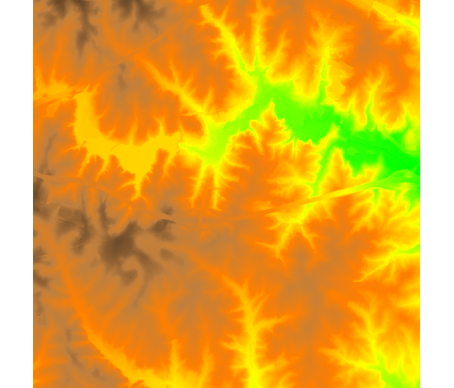
\includegraphics[width=\textwidth]{report_template_image}
    \caption{}
%     \label{fig:afigure}
  \end{subfigure}%
  ~ % ~, \quad, \qquad etc. or \\
  \begin{subfigure}[b]{\twobytwoimgwidth}
    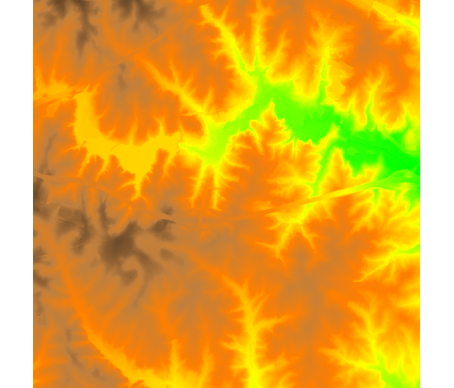
\includegraphics[width=\textwidth]{report_template_image}
    \caption{}
%     \label{fig:}
  \end{subfigure}
  \\[0.01\textheight]
    \begin{subfigure}[b]{\twobytwoimgwidth}
    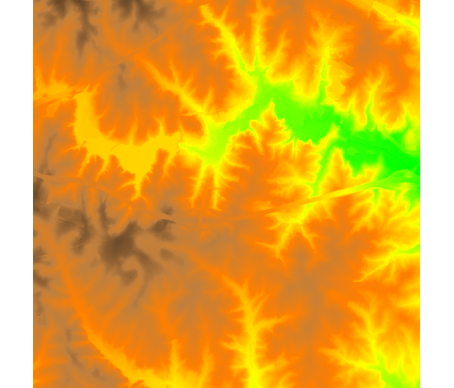
\includegraphics[width=\textwidth]{report_template_image}
    \caption{}
%     \label{fig:}
  \end{subfigure}
  ~
  \begin{subfigure}[b]{\twobytwoimgwidth}
    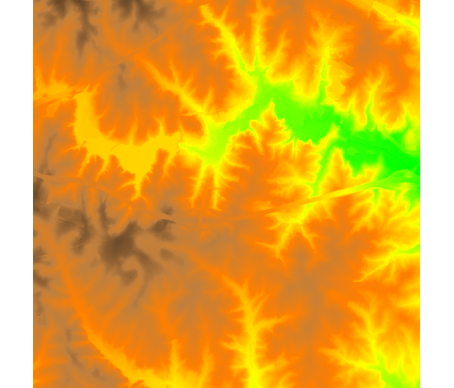
\includegraphics[width=\textwidth]{report_template_image}
    \caption{}
%     \label{fig:}
  \end{subfigure}%
  \caption{A figure with four subfigures (images).
    Note that the black boxes are coming from the demo mode of graphicx package
    and should be disabled for the actual report}
  \label{fig:afigure}
\end{figure}

The elevation and road map for the study area is in the Fig. 1\ldots\ The state wide DEM
and climate data points are in Fig. 10\ldots \emph{(See the page \pageref{fig:figure-internal-label} and further
for suggestion on how to arrange your figures. Two images in row are usually the right choice,
e.g. figure \ref{fig:twotwo})}

We set the computational region to match the raster elevation
\emph{(When showing textual output of a module, use environment verbatim which uses monospace font)}:
\begin{verbatim}
projection: 99 (Lambert Conformal Conic)
zone:       0
datum:      nad83
ellipsoid:  a=6378137 es=0.006694380022900787
north:      734132.59185159
south:      731672.4061379
west:       2092185.68036389
east:       2094646.84229405
nsres:      6.00045296
ewres:      6.00283398
rows:       410
cols:       410
cells:      168100
\end{verbatim}
For emphasis use \verb|\emph{...}| command and for short text which should be shown
verbatim in monospace font use command \verb|\verb+...+| or \verb+\verb|...|+.
Remove \verb|[demo]| from the \verb|\usepackage[demo]{graphicx}| command
to make the actual images show.

%%%%%%%%%%%%%%%%%%%%%%%%%%%%%%%%%%%%%%%%%%%%%%%%%%%%%%%%%%%%%%%%%%%%%%%%%%%%%%%
\section*{Discussion}

Displaying the data in both systems was straightforward. The default color table
for the elevation data was fuzzy, classification into fewer discrete classes
in ArcGIS or conversion to integers brings out the contours (choropleths?).
More detailed representation was achieved by relief shading.
I could get GRASS to display points using the circle symbol --- I was getting the following error.
It was impossible to find where to set the resolution when displaying the elevation data in ArcGIS\ldots


%%%%%%%%%%%%%%%%%%%%%%%%%%%%%%%%%%%%%%%%%%%%%%%%%%%%%%%%%%%%%%%%%%%%%%%%%%%%%%%
\section*{What I learned}

I got familiar with GRASS basics and with the data set.
I learned how to identify the resolution of my raster data in ArcGIS
and that it can be different from the resolution of the displayed raster.

% more templates to include figures
\begin{figure}[htbp]
  \centering
  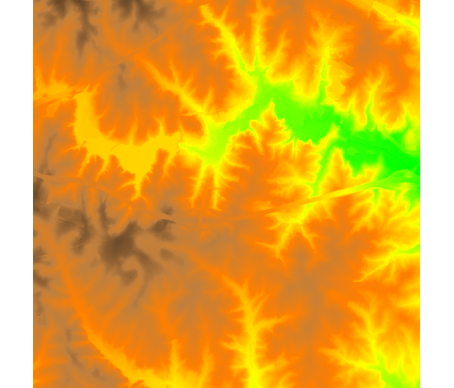
\includegraphics[width=\oneimgwidth]{report_template_image}
  \caption{Image description}
  \label{fig:figure-internal-label}
\end{figure}

\begin{figure}[htbp]
  \centering
  \begin{subfigure}[b]{\twoimgwidth}
    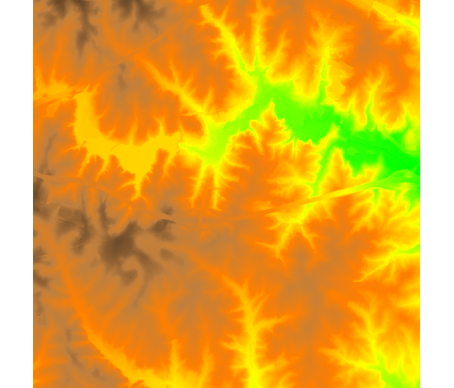
\includegraphics[width=\textwidth]{report_template_image}
    \caption{Left figure}
%     \label{fig:}
  \end{subfigure}%
  ~ % ~, \quad, \qquad etc. or \\
  \begin{subfigure}[b]{\twoimgwidth}
    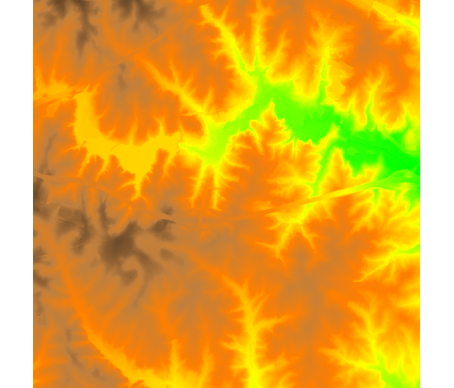
\includegraphics[width=\textwidth]{report_template_image}
    \caption{Right figure}
%     \label{fig:}
  \end{subfigure}
  \caption{Main figure description}
  \label{fig:twotwo}
\end{figure}

\end{document}
